\documentclass[aspectratio=169]{beamer}
\usepackage{soul}
\usepackage{hyperref}

\usepackage{res/beamerouterthememodsplit}
% \useoutertheme{split}
\useinnertheme{circles}
\usecolortheme{whale}
\usecolortheme{orchid}

\setbeamerfont{block title}{size={}}





% Page Numbering
\newcommand*\oldmacro{}%
\let\oldmacro\insertshorttitle%
\renewcommand*\insertshorttitle{%
	\oldmacro\hfill%
	\insertframenumber\,/\,\inserttotalframenumber}

\def\note#1{\ifhidenotes\relax\else\textcolor{blue}{#1}\fi}
\def\anim#1{\ifhideanims\relax\else{#1}\fi}

\setbeamertemplate{naviagation symbols}{}
\setbeamertemplate{frametitle}{}

% \setbeamertemplate{frametitle}{%
% 	\nointerlineskip%
% 	\begin{beamercolorbox}[wd=\paperwidth,ht=1.4ex,dp=0.6ex]{frametitle}
% 		\hspace*{1ex}\insertframetitle%
% 	\end{beamercolorbox}%
% }

%\author{Rory McDaniel, Meriel von Stein}
\title{Computer Science Graduate Student Group \\ (CSGSG)}
\date{August 18, 2023}

\begin{document}

\begin{frame}[plain]
	\maketitle
\end{frame}

\section{CSGSG}

\subsection{Purpose}
\begin{frame}{Purpose}
Officially: 
\begin{itemize}
    \item Provide student representation in the department
    \item Facilitate department-student communication 
\end{itemize}
Generally:
\begin{itemize}
    \item Make life easier for grad students
    \item Help grad students be more successful 
\end{itemize}
\end{frame}

\subsection{People}
\begin{frame}{People}
    \centering\includegraphics[width=\textwidth]{people.PNG}
\end{frame}



\subsection{Spaces}
\begin{frame}{Spaces}
\begin{itemize}
    \item CS Grad Lounge: Rice 434
    \item Discord: \url{https://discord.gg/rmdAP32E2g}
    \item \url{https://csgsg.org/}
    \item Temporary prayer hall - Students can temporarily use MEC 206 and Thornton D102.
\end{itemize}
\end{frame}

\subsection{Recruiting}
\begin{frame}{Recruiting}
Why:
\begin{itemize}
    \item Amazing on CV
    \item Learn about the department (and academia in general)
    \item Practice leadership, mentoring and organization skills
\end{itemize}
Eligibility:
\begin{itemize}
    \item Any grad student in CS or CpE can be an officer
    \item Officers are elected by CS/CpE grad student body 
    \item Terms run by calendar year
    \\ (So MS/MCS students would need to run this Nov/Dec.)
\end{itemize}
\end{frame}

\subsection{Events}
\begin{frame}{Events}
\begin{columns}
\begin{column}{0.5\textwidth}
CSGSG Social Events:
\begin{itemize}
    \item Run by the CSGSG Social Chairs: Matt \& Anshuman
    \item Our goal is to run 2 events a month: one free food during a week, one large event on a weekend.
    \item Events are free to CS and CPE students. 
    \item Seats are generally first come first serve. 
\end{itemize}
\end{column}

\begin{column}{0.5\textwidth}
Upcoming Events:
\begin{itemize}
    \item Tuesday 8/22 (1st day of classes): Mezeh for lunch!
    \item Saturday 8/26: "Beach" Day at Walnut Creek
\end{itemize}
Signups are in your email, or signup here:

 \begin{figure}
     \centering
     
\includegraphics[width=0.7\textwidth]{QRs.pdf}
 \end{figure}
\end{column}
\end{columns}
\end{frame}


\subsection{Mentorship Program}
\begin{frame}{Mentorship Program}
\begin{columns}
\begin{column}{0.5\textwidth}
\textbf{What is the mentorship program?}
The mentorship program is a way for new students to acclimate to the UVA CS/CpE department and graduate life, and for established students to gain mentoring and leadership experience.

\vspace{0.33cm}

If you're thinking of becoming a part of CSGSG, this is a good program to participate in.
\end{column}
\begin{column}{0.5\textwidth}  %%<--- here
    \begin{center}
    Link to sign-up:
    
     
\includegraphics[width=0.5\textwidth]{mentor-program-fall2023.png}

     {Or search ``cs-grads'' in your email}
     \end{center}
\end{column}
\end{columns}
\end{frame}




% 

\subsection{Research Symposium}
\begin{frame}{Research Symposium}
\begin{itemize}
    \item Researchers gather to present their research in the form of presentations, posters, and panel discussions.
    \item Platform for all UVA students to showcase their research, obtain constructive feedback on research projects, and promote networking.
    \item Event date: Tuesday, Oct 3, 2023
    \item Location: Rice 130
    \item Participation in the Symposium and engagement in poster presentations are highly encouraged for first-year students.
\end{itemize}
\end{frame}


\section{Program Info}

\subsection{Rotations}

\begin{frame}{Rotations}
Why:
\begin{itemize}
    \item Finding a good match
    \item Finding co-advisors
    \item Finding backups
    \item Finding committee members for quals (PhD students) or thesis (MS students)
\end{itemize}
You can do all \st{3} \textbf{2 rotations} without repercussions. 
\begin{itemize}
    \item If you feel this isn't the case, please let us know (see ''Useful Contacts'' slide).
    \item The department spends a lot of money to make sure you get this opportunity.
\end{itemize}
\end{frame}

\subsection{Finding an Advisor}
\begin{frame}{Finding an Advisor}
\noindent ``How do I choose my advisor?'' is one of the most frequent questions we get.

Your advisor is one of the most significant contributing factors to your PhD.


\vspace{0.33cm}
{\scriptsize
\begin{itemize}
    % \item \href{https://www.example.com}{{\underline{\textcolor{blue}{link}}}}
    \item \textbf{CRA-Widening Participation:} \href{https://acrobat.adobe.com/link/track?uri=urn:aaid:scds:US:5d051a05-acc1-3778-975f-a84d9553c2b1}{{\underline{\textcolor{blue}{Finding an Advisor and Developing an Effective Working}} {\underline{\textcolor{blue} {Relationship with Them}}}}}
    
    \item \textbf{CRA-Widening Participation:} \href{https://cra.org/cra-wp/wp-content/uploads/sites/8/2022/04/Advising_Relationship.pdf}{{\underline{\textcolor{blue}{How to Make the Most of Student-Advisor Relationships}}}}
    \item \textbf{IEEE:} \href{https://ieeexplore.ieee.org/stamp/stamp.jsp?tp=&arnumber=1033661}{\underline{\textcolor{blue}{E. K. Miller, "Choosing a grad school advisor," in IEEE Potentials, vol. 21, no. 3, pp.}} \underline{\textcolor{blue}{21-23, Aug.-Sept. 2002, doi: 10.1109/MP.2002.1033661.}}}
    \item \textbf{NATURE Journal:} \href{https://www.nature.com/articles/d41586-021-03703-z}{\underline{\textcolor{blue}{Managing up: how to communicate effectively with your PhD advisor}}}
    \item \textbf{Columbia University:} \href{https://www.cs.columbia.edu/wp-content/uploads/2019/03/Get-Advisor.pdf}{\underline{\textcolor{blue}{The Definitive ‘what do I ask/look for’ in a PhD Advisor Guide}} 
    \underline{\textcolor{blue}{(minus lifestyle questions)}}}
    \item \textbf{Virginia Tech:} \href{https://www.graduate.ombudsman.vt.edu/disrupting_academic_bullying.html}{\underline{\textcolor{blue}{Disrupting Academic Bullying}}}
\end{itemize}
}




\end{frame}


\subsection{PhD Stipends}
\begin{frame}{PhD Stipends}
\begin{columns}
\begin{column}{0.3\textwidth}
\footnotesize{
Fall 2023:

\begin{itemize}
\item Tier1: \$35,022 (+5.9\%)
\item Tier2: \$36,504 (+3.3\%)
\item Tier3: \$38,012 (+1.3\%)
\end{itemize}
}

Fall 2022: (no increase)
\footnotesize{
\begin{itemize}
\item Tier1: \$33,072 
\item Tier2: \$35,334 
\item Tier3: \$37,518 
\end{itemize}
}

Fall 2021: 
\footnotesize{
\begin{itemize}
\item Tier1: \$33,072 
\item Tier2: \$35,334 
\item Tier3: \$37,518 
\end{itemize}
}
\end{column}
\begin{column}{0.7\textwidth}  %%<--- here
    \begin{center}
     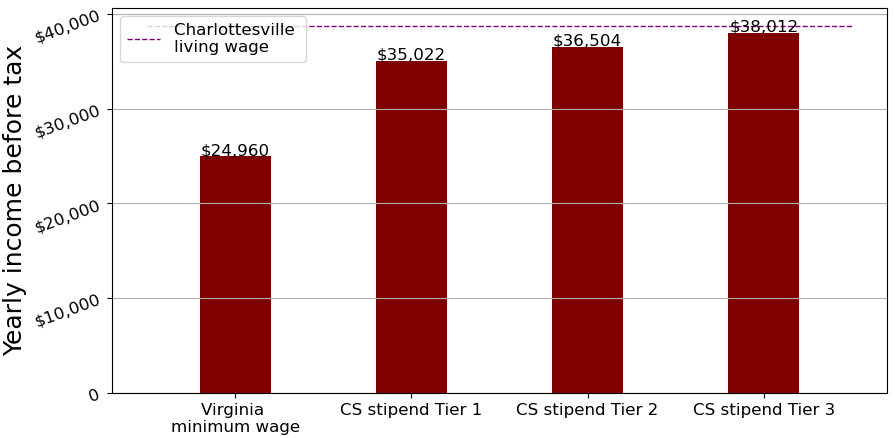
\includegraphics[width=1.\textwidth]{temp-EHLLMO.png}   
     {\footnotesize Lowest living wage for Charlottesville, VA is \textbf{\$38,688} for a single adult with no dependents.}
     {\tiny Source: Glasmeier, Amy K. Living Wage Calculator. 2023. Massachusetts Institute of Technology. https://livingwage.mit.edu.}
     \end{center}
\end{column}
\end{columns}
\end{frame}

\section{Resources}
\subsection{Mental Health}
\begin{frame}{Mental Health}
Grad students as a group are well known to have significantly higher mental health issues than the general population. \\
This is perfectly logical and expected - we self-select highly driven people and then put them in incredibly stressful roles.
\begin{itemize}
    \item Counseling \& Psychological Services (CAPS)
    \\ \url{https://www.studenthealth.virginia.edu/CAPS}
    \item Maxine Platzer Lynn Women's Center
    \\ \url{https://womenscenter.virginia.edu/}
\end{itemize}
\end{frame}


\subsection{Useful Contacts}
\begin{frame}{Useful Contacts}
\begin{itemize}
    \item Department Office
    \\ \url{cs-office@virginia.edu}
    \item Department Ombuds (Sebastian Elbaum)
    \\ \url{selbaum@virginia.edu}
    \item University Ombuds
    \\ \url{https://eocr.virginia.edu/ombuds}
    \item CSGSG General
    \\ \href{https://discord.gg/rmdAP32E2g}{Discord} or \url{csgsg@virginia.edu} or anonymous form on \url{https://csgsg.org}
    \item CSGSG Chair (Nusrat Jahan Mozumoder)
    \\ \href{https://discord.gg/rmdAP32E2g}{Discord} or \url{nm8tm@virginia.edu}
    \item CSGSG Mentoring Rep (Meriel von Stein)
    \\ \href{https://discord.gg/rmdAP32E2g}{Discord} or \url{meriel@virginia.edu}
    
\end{itemize}
\end{frame}

\subsection{Additional Resources}
\begin{frame}{Additional Resources}
\begin{itemize}
    \item \textbf{CRA-Widening Participation:} \href{https://cra.org/cra-wp/wp-content/uploads/sites/8/2022/03/Balancing-Grad-School-and-Life.pdf}{\underline{\textcolor{blue}{Balancing Graduate School and Personal Life}}}

    \item \textbf{CRA-Widening Participation:} \href{https://acrobat.adobe.com/link/track?uri=urn:aaid:scds:US:8dae44ac-ea20-3fa7-8cac-4f8ceea0d039}{\underline{\textcolor{blue}{Building Resiliency \& Overcoming Failure}}}
    
    \item \textbf{Carnegie Mellon University:} \href{https://blog.ml.cmu.edu/2020/03/02/questions-to-ask-a-prospective-ph-d-advisor-on-visit-day-with-thorough-and-forthright-explanations/}{\underline{\textcolor{blue}{Questions to Ask a Prospective Ph.D. Advisor on}} \underline{\textcolor{blue}{Visit Day, With Thorough and Forthright Explanations}}}
    
    \item Matt Might's \href{https://matt.might.net/articles/}{\underline{\textcolor{blue}{blog}}}

    \item \href{https://phdcomics.com/}{phdcomics.com}

\end{itemize}
\end{frame}

\subsection{Questions?}
\begin{frame}{Questions?}
\begin{itemize}
    \item Please let us know if you have questions!
    \item You can ask now, find us during lunch, email us, or ask over the discord.
\end{itemize}
\end{frame}

\end{document}